\section{Application to an e-governance workload, and limitations}
\label{sec:case}

We instantiate Problem~\ref{prob:sizing} on a national-scale profile:
approximately $3.0\times10^{7}$ ballots over a twelve-hour window, with a peak
window concentrating about a quarter of the daily volume and therefore a peak
demand $\Dpk\approx2.1\times10^{3}$ transactions per second. The safety
requirement is that a coordinated omission fault affecting one fifth of the
validators be detected within one epoch with probability at least $1-\epss$.

Because the bi-factor law is calibrated on \RNM{}-normalized throughput
$\TPSn=\TPS/\q$, absolute demand and the fitted law live in different units.
We therefore introduce an explicit production scale-up $\kappaScale$ such that
the absolute predictor is $\kappaScale\cdot\widehat{\TPSn}(\n,\cc)$. The default
reported here is the \emph{minimal admissible} scale: the smallest
$\kappaScale$ for which the lower prediction bound at $\n=4$ meets $\Dpk$
(hardware just capable of serving the peak at the smallest QBFT validator
set). With that $\kappaScale=\resKappa$ and operating concurrency
$\cc^{\star}=\resCstar$, Theorem~\ref{thm:window} yields the feasibility
window $[\resNminCase,\resNmaxCase]$ and the recommendation
$\nopt=\resNoptCase$; Figure~\ref{fig:window} shows the two constraints and
their intersection. Detector rates enter at the Youden-optimal participation
threshold $\thr=\resDetectorThr$ of experiment~X5.

\begin{figure}[!t]
\centering
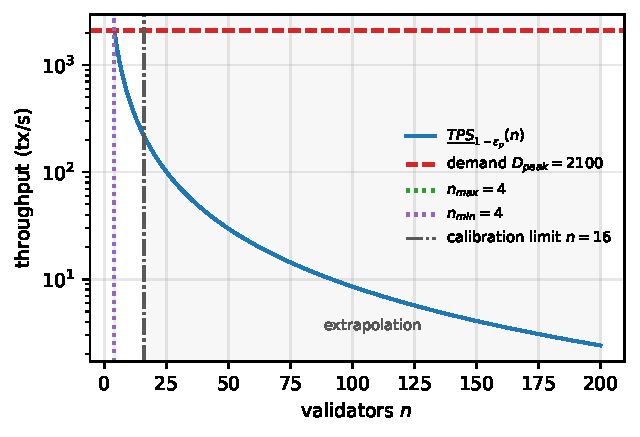
\includegraphics[width=0.78\textwidth]{figures/fig_window}
\caption{Feasibility window. The solid curve is the confidence-adjusted
absolute throughput $\kappaScale\cdot\underline{\TPSn}_{1-\epsp}(\n)$ against
the demand $\Dpk$; the shaded band marks the admissible interval
$[\nmin,\nmax]=[\resNminCase,\resNmaxCase]$ at the minimal admissible
$\kappaScale=\resKappa$}
\label{fig:window}
\end{figure}

The width of the window is the design margin, and it responds to four factors. A
relative change in $\beta$ shifts $\log\nmax$ by
$-\log\nmax\,\Delta\beta/\beta$, so the upper endpoint is most sensitive
precisely when the deployment sits far above the calibration range. Increasing
$\rho$ inflates $\nmin$ proportionally to $1+(\kf-1)\rho$
by~\eqref{eq:nmin}, so strongly coordinated faults can close the window on their
own. Using $\beta(\mathrm{RTT})$ from experiment~X4 lowers $\nmax$, which is the
price of geographic distribution. And tightening $\epsp$ lowers $\nmax$ while
tightening $\epss$ raises $\nmin$: the window closes from both sides as the
system is made more conservative. The analysis thus produces an operational
statement of the form: \emph{with confidence $1-\epsp$ the network sustains the
peak demand up to $\nmax$ validators, and detects the specified coordinated
fault with probability at least $1-\epss$ from $\nmin$ upward; the cheapest
admissible configuration is $\nopt$; the required production scale relative to
the \RNM{} unit is $\kappaScale$}.

\begin{Remark}
This case study illustrates the sizing workflow. It is not a recommendation to
conduct binding elections on a blockchain: the consensus layer addresses neither
endpoint compromise nor coercion~\cite{springall2014,specter2020,park2021}. The
same workflow applies unchanged to registry and identity workloads, where those
objections do not arise.
\end{Remark}

\subsection{Limitations}
\label{sec:limitations}

\paragraph{Fault class.}
The peer-to-peer transport is encrypted, so network-level injection cannot be
selective with respect to consensus message type. Experiment~X5 therefore
realizes omission and duplication faults only, excluding equivocation and
signature forgery, and every statement about $\pd$, $\pf$ and $\pmiss$ is
conditional on that class. Empirically, signer-metrics detection of this class
is weak (AUC~$\resAuc$ at the Youden threshold $\thr=\resDetectorThr$): the
safety constraint is consequently non-binding at the operating point of
Section~\ref{sec:case}, and the window is set by throughput.

\paragraph{Absolute throughput and measured range.}
Under the \RNM{} protocol each validator receives a small fixed CPU quota, so
absolute throughput is far below what dedicated hardware would deliver and is
not comparable with published benchmarks; every claim here concerns exponents,
coverage and the sizing decisions derived from them, and
Statement~\ref{st:qinvariance} is what licenses that separation. Absolute demand
enters the sizing problem only through the explicit scale-up $\kappaScale$ of
Problem~\ref{prob:sizing}. The largest directly measured validator set is
bounded by host memory, and extrapolation beyond it rests on the calibrated
model and on simulation; the intervals of Statement~\ref{st:pi} quantify, but
do not eliminate, the associated risk. The fitted consensus exponent
$\beta=\resBeta$ is steep, so even at the minimal admissible $\kappaScale$ the
feasibility window collapses to a single point $\n=\resNoptCase$: that is a
substantive sizing conclusion, not a numerical artefact.

\paragraph{Single host and single platform.}
All measurements come from one host and one implementation, with wide-area
behaviour emulated rather than observed. The contributions are not equally
exposed. Theorem~\ref{thm:identifiability} is a statement about least squares
and does not depend on the platform; what depends on it are the values of
$\beta$ and $\gamma$. Experiment~X9 was intended to falsify the
path-re-sampling prediction on a second QBFT-family client, but that arm of the
campaign did not produce usable records, so the numerical coefficients remain
Besu-specific. The \RNM{} protocol is more exposed, since
Assumption~\ref{as:separable} concerns the scheduler and the runtime: the X2
partial $F$-test rejects exact quota invariance on $\{0.20,0.25,0.33\}$, and we
therefore report the bi-factor fit at the reference quota $\q=0.25$ rather than
pooling across quotas.

\paragraph{Asymmetry between theory and measurement.}
The analytical part of this work is more complete than the empirical part. The
theorems hold as stated; the calibrated coefficients rest on a campaign bounded
by what a four-core runner can host, and Assumption~\ref{as:separable} in
particular is supported over a narrow quota range. The numerical values should
be read as provisional and the structural claims --- the form of the bias, the
shape of the feasible set --- as the durable part. The exchangeable correlation
of Assumption~\ref{as:rho} and the approximate log-normality underlying
Statement~\ref{st:pi} are likewise approximations, each accompanied by a test;
where a test rejects, the corresponding claim is restricted rather than
retained. Finally, Theorem~\ref{thm:window} assumes only that $\Cost$ is
nondecreasing, so deployments with non-monotone institutional cost fall outside
it, although the window itself remains valid.
